\documentclass{beamer}
\usepackage{amssymb}
\usepackage{amsmath}
\usepackage{commath}
\usepackage{amsthm}
\usepackage{lmodern}
\usepackage{scrextend}
\usepackage{xcolor}
\newcommand*\diff{\mathop{}\!\mathrm{d}}
\usetheme{Luebeck}
\useoutertheme[subsection=false, footline=authortitle]{miniframes}
\usecolortheme{crane}

\title{The polluted atmosphere as a shallow domain}
\author[N\'ora Juh\'asz]{N\'ora Juh\'asz \\[1mm] in collaboration with Prof. Donatella Donatelli}
\institute{Department of Information Engineering, Computer Science and Mathematics \\ University of L'Aquila }

\date{16th May, 2019}

\logo{
    
\includegraphics[width=1cm,height=1cm,keepaspectratio]{LogoModCompShock.jpg}\hspace*{10.5cm}~%
    
\includegraphics[width=1cm,height=1cm,keepaspectratio]{LogoDisim.png}~%
}

\begin{document}

\begin{frame}
\titlepage
\end{frame}

\section{Local geophysical coordinate system}

%%% TEXT: 1) low Mach number: Boussinesq approximation, constant density. it is the conservation of mass eq. that becomes the div-free condition through the Boussinesq approximation. density taken to be identically equal to one
%%% 2) Note: full, complete. basic conservation of momentum.
%%% 3.) A superior method to model diffusion in complex scenarios is to use the diffusion tensor, a 3 x 3 array of numbers corresponding to diffusion rates in each combination of directions. The three diagonal elements (Dxx, Dyy, Dzz) represent diffusion coefficients measured along each of the principal (x-, y- and z-) laboratory axes. The six off-diagonal terms (Dxy, Dyz, etc) reflect reflect the correlation of random motions between each pair of principal directions.
%%% 4.) Taking this general concept as foundation, a first idea to create a theoretically correct model for the polluted atmosphere on Earth is to take exactly this classical concept.
\begin{frame}{Start: 3D Navier-Stokes}

\textbf{Starting point:} fluid dynamics fact --- wind flow on the globe is governed by the 3D incompressible Navier-Stokes equations.

\textbf{Result:} 

\setbeamertemplate{itemize items}[circle]
  \begin{itemize}
    \item the 3D incompressible Navier-Stokes equation, and 
    \item a convection-diffusion equation to describe the pollution effect
  \end{itemize}
  
%%% fluid velocity    
$$ \partial_t \mathbf{v} + (\mathbf{v} \cdot \nabla)\mathbf{v} -\Delta_{\nu} \mathbf{v} + \nabla q + 2 \mathbf{w} \times \mathbf{v}= \mathbf{g} $$
    
$$ \nabla \cdot \mathbf{v} = 0 $$
    
%%% representing pollutants in the atmosphere
$$ \partial_t P + \mathbf{v} \cdot \nabla P = \nabla \cdot (\mathbf{K} \nabla P) + Q $$

\end{frame}

%%% TEXT: Central component for describing the dynamics of geophysical fluids: hydrostatic approximation. In the vertical dimension we simply use the formula describing the hydrostatic pressure, instead of the complete momentum equation.
\begin{frame}{Hydrostatic approximation}

\textbf{Point of apparent theoretical conflict:} The previously described model is \textbf{not} what is widely used in meteorology and oceanology to describe geophysical processes.

The fundamental equations in meteorology --- primitive equations. 

%%% horizontal fluid velocity    
$$ \partial_t \mathbf{v}_H + \mathbf{v}_H \cdot \nabla_H \mathbf{v}_H + v_3 \partial_z \mathbf{v}_H - \Delta_{\nu} \mathbf{v}_H + \nabla_H q + 2 (\mathbf{w} \times \mathbf{v})_H = 0 $$

%% hydrostatic pressure
$$ \frac{\partial q}{\partial z} = - \mathbf{g}$$

%% divergence-free condition
$$ \nabla \cdot \mathbf{v} = 0 $$
    
%%% representing pollutants in the atmosphere
$$ \partial_t P + \mathbf{v} \cdot \nabla P = \nabla \cdot (\mathbf{K} \nabla P) + Q $$

\begin{center}
\textit{Experience shows:} This natural simplification is highly

accurate for large-scale fluids. 
\end{center}

\end{frame}

%%% TEXT: 1.) Our goal is to provide a rigorous analytical proof that this approximation is mathematically acceptable.
%%% 2.) The way we do this: we start by incorporating the concept of shallowness into the model and see what happens to the starting point model if we take the aspect ratio parameter closer and closer to 0 --- we will find that the two models are connected not just formally through this parameter, but also on the level of weak solutions.
%%% 3.) Augmented pressure concept.
%%% 4.) An analytical proof that shows that this asymptotic limit model is meaningfully and rigorously connected to the original one in the case of large-scale geological fluids.
\begin{frame}

\textbf{A natural question to ask:} 

\begin{enumerate}
  \item Is this valid?
  \item What makes it valid?
\end{enumerate}

\textbf{Justification:} An analytical proof.

\setbeamertemplate{itemize items}[circle]
\begin{itemize}

  \item The key to the justification process is to take this following phrase: \textbf{\textit{"we are considering a large-scale geophysical fluid on the surface of the Earth,"}} and to include its meaning into the model in mathematical terms.

  \item Scale analysis will show that the dominant term in the full vertical momentum equation is $\frac{\partial q}{\partial z}$ and the gravity term, resulting in the hydrostatic approximation.

\end{itemize}

\end{frame}

%%% TEXT: 1.) Before describing the scaling process, first of all we fix a coordinate system. We use a local Cartesian coordinate system 
%%% 2.) "locally" - it means however the surface of a few countries
%%% 3.) Here the x axis is perpendicular to the Earth rotation vector, this makes the Coriolis term more simple.
\begin{frame}{Local geophysical coordinate system}

\textbf{"$\beta$-plane approximation"} $\to$ this means that we can neglect the curvature of the Earth, and thus is valid locally.

{Geophysical rotating frame:}

\begin{itemize}
\item $z$ --- vertical coordinate ("upwards"),
\item $x$ --- east,
\item $y$ --- north.
\end{itemize}

This is an often used coordinate system choice as the Coriolis term takes a rather simple form expressed in these coordinates.

\end{frame}

%%% TEXT: 1.) make the domain independent from epsilon by using the physical dimensions.
%%% 2.) epsilon incorporates the shallowness in a mathematical way
\begin{frame}{Scaling - part 1}

Geophysical fluid $\to$ shallow domain characteristics --- the domain is greater horizontally than in the vertical dimension.

One of the main tools to exploit the "almost" 2D structure of the atmosphere:

$$\epsilon = \frac{\text{characteristic depth}}{\text{characteristic width}} = \text{aspect ratio}.$$

\textbf{Natural scaling process:}

\begin{enumerate}
    \item $ x=x_1, y=x_2, z=\epsilon x_3 $
    \item $ v_1 = u_1^{\epsilon}, v_2 = u_2^{\epsilon}, v_3 = \epsilon u_3^{\epsilon}, p = p^{\epsilon}, $
    \item $ P = \frac{1}{\epsilon} C^\epsilon, Q = \frac{1}{\epsilon} S^\epsilon. $

\end{enumerate}

\end{frame}

%%% TEXT: 1.) the physical dimension of viscosity and diffusivity
%%% 2.) If we consider only the scaling part introduced until now, we are still ignoring a complexity, which not just would be overly simplistic, but it is the inclusion of this following specific feature that makes it possible for the proof to work.

\begin{frame}{Scaling - part 2}
We need to consider the highly anisotropic nature of viscosity and diffusivity $\to$ this means that these rates are strongly different in horizontal and vertical directions.
Rescaling these parameters according to the largely different scales:

  \begin{enumerate}
    \item $ \nu_x = \nu_1, \quad \nu_y = \nu_2 , \quad \nu_z = \epsilon ^ 2\nu_3, $
    \item
     \begin{gather}
      \begin{bmatrix} K_{xx} & K_{xy} & K_{xz} \\ K_{yx} & K_{yy} & K_{yz} \\ K_{zx} & K_{zy} & K_{zz} \end{bmatrix}
       =
      \begin{bmatrix}
    M_{11} & M_{12} & \epsilon M_{13} \\ M_{21} & M_{22} & \epsilon M_{23} \\ \epsilon M_{31} & \epsilon M_{32} & \epsilon^2 M_{33}
  \end{bmatrix} \nonumber
\end{gather}
  \end{enumerate}
  
The diffusivity matrix is assumed to be coercive.

\end{frame}


%%% TEXT: 1.)  For modelling the source function of the concentration we use the Gaussian impulse approach.
%%% 2.) We use a parametrised nascent delta function to describe the source term, with the parameter being $\epsilon$.
\begin{frame}{Source term}

$$S_\epsilon (t, t_s, x, x_s) = s(t, t_s) \delta_\epsilon (x - x_s),$$

with the activation term \center{$s(t,t_s)= IH(t - t_s)$.}

\setbeamertemplate{itemize items}[circle]
\begin{itemize}

  \item $\delta_\epsilon$ is a nascent delta function,
  \item $H(\cdot)$ is the Heaviside step function,
  \item $I$ is the intensity of the source.

\end{itemize}

In the limit model we naturally arrive to the delta distribution as a source.

\end{frame}

%%% TEXT: 1.) How the two models will eventually look like when we write them out in detail, including the following specific ideas that we also use combined to the main, general foundation of the model, such as using a Gaussian pulse as a source term.
%%% 2.) Why do we have an epsilon^2 on the third equation: the second epsilon comes from the denominator of the pressure term (there is a vertical derivative)
%%% 3.) Point out the disappearing control on u_3
\begin{frame}{Anisotropic equations}

  In $\Omega \times (0,T)$ we have the following system.

    \[ \partial_t u^\epsilon _1 + \mathbf{u}^\epsilon \cdot \nabla u^\epsilon _1 -\Delta_\nu u^\epsilon _1 -\alpha u_2^\epsilon + \epsilon \beta u_3^\epsilon + \partial_1 p^\epsilon = 0 \]
    
    \[ \partial_t u_2^\epsilon + \mathbf{u}^\epsilon \cdot \nabla u_2^\epsilon -\Delta_\nu u_2^\epsilon + \alpha u_1^\epsilon + \partial_2 p^\epsilon = 0 \]
    
    \[\epsilon^2 \{  \partial_t u_3^\epsilon + \mathbf{u}^\epsilon \cdot \nabla u_3^\epsilon -\Delta_\nu u_3^{\epsilon} \} - \epsilon \beta u_1^\epsilon + \partial_3 p^\epsilon = 0 \]
    
    \[ \nabla \cdot \mathbf{u}^\epsilon= 0  \]
    
    \[ \partial_t C^\epsilon + \mathbf{u^\epsilon} \cdot \nabla C^\epsilon = \nabla \cdot (\mathbf{M} \nabla C^\epsilon) + S^\epsilon \]
    
\end{frame}

\begin{frame}{Local domain and boundary conditions}
  \begin{figure}
    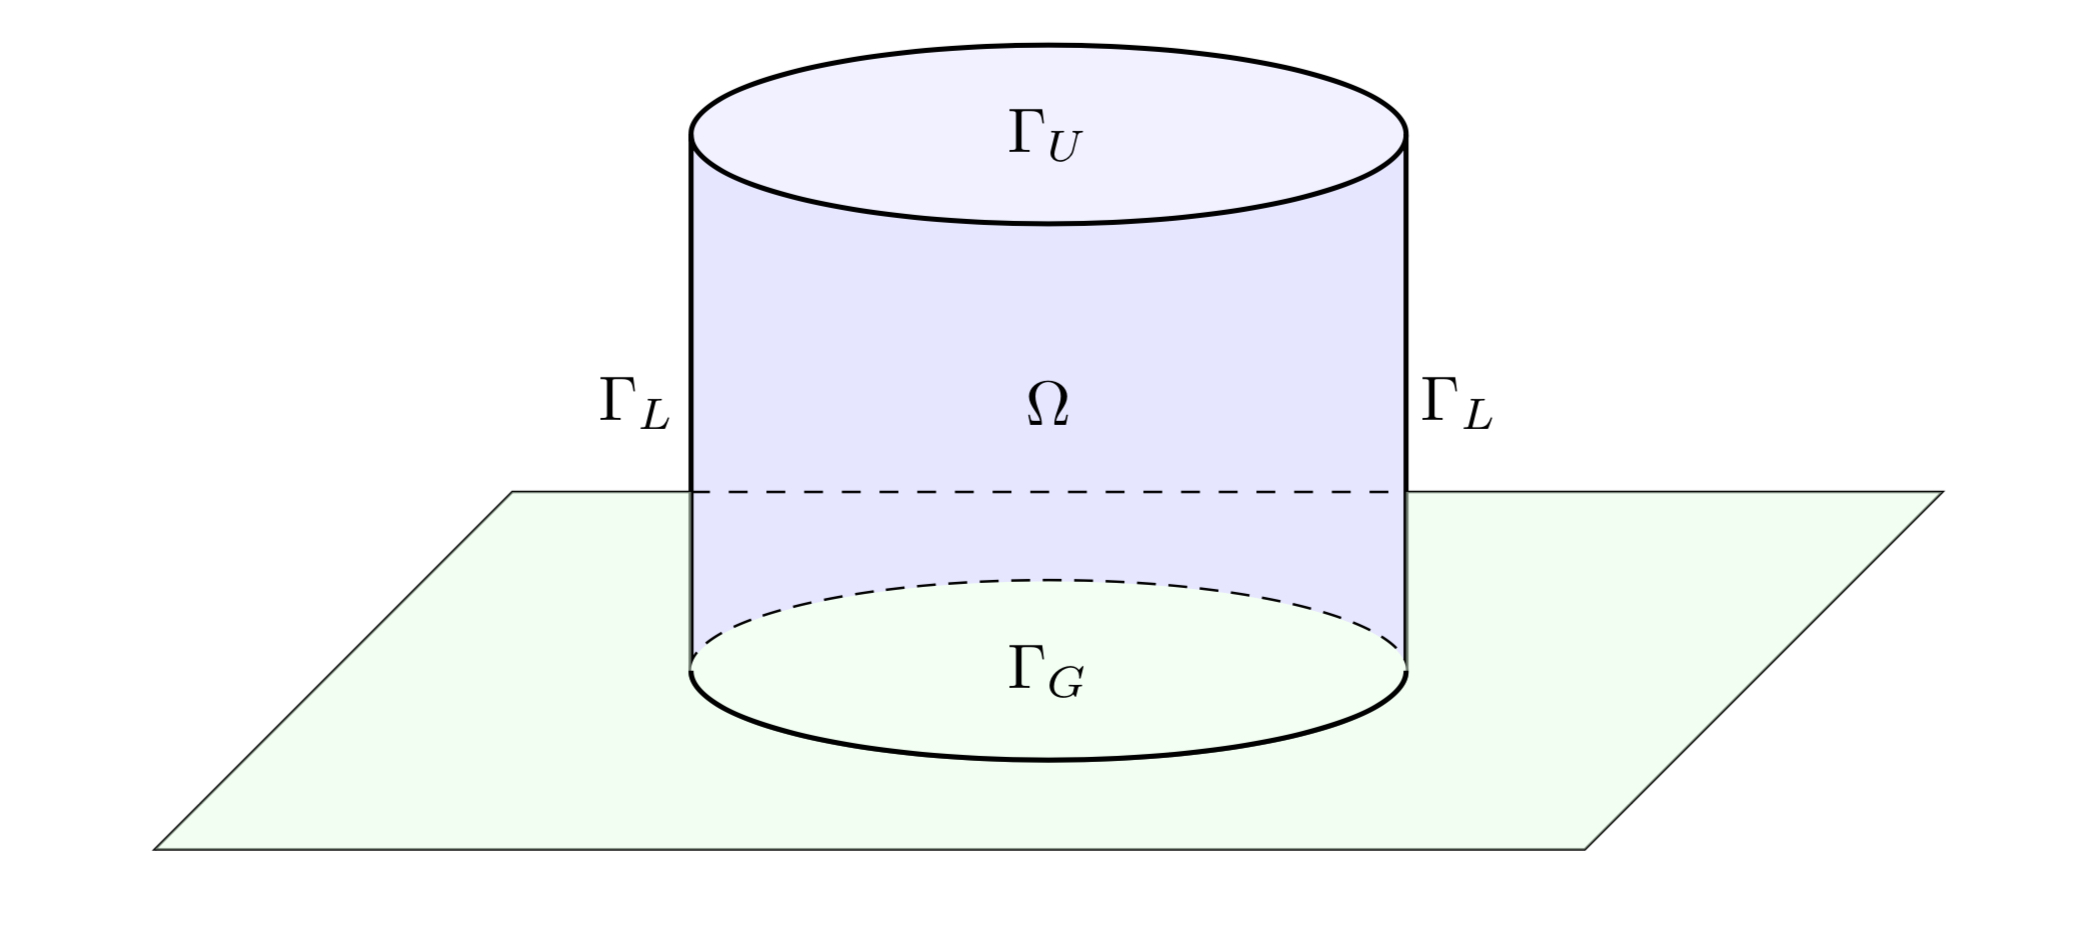
\includegraphics[width=\linewidth]{domain.jpg}
    \caption{A local slice of the atmosphere}
    \label{fig:atmosphere}
  \end{figure}
\end{frame}

\begin{frame}{Anisotropic equations - Part 2}

  The initial and boundary conditions are chosen to be

    $$ \mathbf{u}^\epsilon (\cdot, t = 0) = \mathbf{u}_0, \quad C^\epsilon (\cdot, t=0) = C_0  \quad \text{ in } \Omega, $$
    $$ \mathbf{u}^\epsilon = 0 \text{ on } \Gamma \times (0,T),$$
    $$ C^\epsilon = 0 \text{ on } ( \Gamma_U \cup \Gamma_L) \times (0,T), $$
    $$ \partial_1 C^\epsilon = \sigma_1, \partial_2 C^\epsilon = \sigma_2,\ \partial_3 C^\epsilon= 0 \text{ on } \Gamma_G \times (0,T), $$
    $$ \boldsymbol{\sigma} = (\sigma_1, \sigma_2, 0) \in L^2(0,T; \Gamma_G) $$

\end{frame}

\begin{frame}{Anisotropic equations}

  In $\Omega \times (0,T)$ we have the following system.

    \[ \partial_t u^\epsilon _1 + \mathbf{u}^\epsilon \cdot \nabla u^\epsilon _1 -\Delta_\nu u^\epsilon _1 -\alpha u_2^\epsilon + \epsilon \beta u_3^\epsilon + \partial_1 p^\epsilon = 0 \]
    
    \[ \partial_t u_2^\epsilon + \mathbf{u}^\epsilon \cdot \nabla u_2^\epsilon -\Delta_\nu u_2^\epsilon + \alpha u_1^\epsilon + \partial_2 p^\epsilon = 0 \]
    
    \[\epsilon^2 \{  \partial_t u_3^\epsilon + \mathbf{u}^\epsilon \cdot \nabla u_3^\epsilon -\Delta_\nu u_3^{\epsilon} \} - \epsilon \beta u_1^\epsilon + \partial_3 p^\epsilon = 0 \]
    
    \[ \nabla \cdot \mathbf{u}^\epsilon= 0  \]
    
    \[ \partial_t C^\epsilon + \mathbf{u^\epsilon} \cdot \nabla C^\epsilon = \nabla \cdot (\mathbf{M} \nabla C^\epsilon) + S^\epsilon \]
    
\end{frame}

\begin{frame}{Hydrostatic equations}
  
    \[ \partial_t u_1 + \mathbf{u} \cdot \nabla u_1 - \Delta_\nu u_1 -\alpha u_2 + \partial_1 p = 0 \text{ in } \Omega \times (0,T) \]
    
    \[ \partial_t u_2 + \mathbf{u} \cdot \nabla u_2 - \Delta_\nu u_2 -\alpha u_1 + \partial_2 p = 0 \text{ in } \Omega \times (0,T) \]
    
    \[ \partial_3 p = 0 \text{ in } \Omega \times (0,T) \]
    
    \[ \nabla \cdot \mathbf{u} = 0 \text{ in } \Omega \times (0,T) \]
    
    \[ \partial_t C + \mathbf{u} \cdot \nabla C = \nabla \cdot (\mathbf{M} \nabla C) + S \text{ in } \Omega \times (0,T) \]
    
    Initial and boundary conditions are analogous except for using $$ u_1 = u_2 = u_3 n_3 = 0 \text{ on } \Gamma \times (0,T). $$

\end{frame}

%%% TEXT: 1.) note the spaces where u^\epsilon and C^\epsilon come from - the "usual" weak solution spaces, added with specialities for BCs
\begin{frame}{Weak formulation - anisotropic system}
\changefontsizes{10pt}
Find $\mathbf{u}^\epsilon$ and $C^\epsilon$, such that
  
  \begin{equation}
    \begin{split} \nonumber
      & \int_0^T \bigg [ -(\mathbf{u}^\epsilon_H, \partial_t \mathbf{\tilde{u}}_H) + (\nabla_\nu \mathbf{u}^\epsilon_H, \nabla_\nu \mathbf{\tilde{u}}_H) - (\mathbf{u}^\epsilon_H, (\mathbf{u}^\epsilon \cdot \nabla) \mathbf{\tilde{u}}_H) + (b(\mathbf{u}^\epsilon_H), \mathbf{\tilde{u}}_H) \bigg ] \diff t \\
      & + \epsilon \beta \int_0 ^ T \big [ (u_3 ^\epsilon, \tilde{u}_1) - (u_1^\epsilon, \tilde{u}_3) \big ] \diff t\\
      & + \epsilon^2 \int _0 ^ T \big [ -(u_3^\epsilon, \partial_t \tilde{u}_3) +(\mathbf{u}^\epsilon \cdot \nabla u_3 ^ \epsilon, \tilde{u}_3) + (\nabla_\nu u_3^\epsilon, \nabla_\nu \tilde{u}_3) \big ] \diff t \\
      & = (\mathbf{u}^\epsilon_{0H}, \mathbf{\tilde{u}}_H(0)) + \epsilon^2 (u_{03}^\epsilon, \tilde{u}_3 (0)) \diff t
    \end{split}
  \end{equation}
  
  and
  
    \begin{equation}
    \begin{split} \nonumber
      & \int_0^T \bigg [ -(C^\epsilon, \partial_t \tilde{C}) -(\mathbf{u}^\epsilon C^\epsilon, \nabla \tilde{C}) + (\mathbf{M} \nabla C^\epsilon, \nabla \tilde{C}) - \int_{\Gamma_G} \boldsymbol{\sigma} \mathbf{M} \tilde{C} \vec{\boldsymbol{n}}_{\Gamma_G} \bigg ] \diff t \\
      & =  (C^\epsilon (0), \tilde{C} (0)) + \int_0^T (S^\epsilon,\tilde{C}) \diff t
    \end{split}
  \end{equation}

\end{frame}

\begin{frame}{Main theorem}

  We show a rigorous connection between the two sets --- taking the limit in the solutions we arrive to a justification of the hydrostatic model for the case of the polluted atmosphere.

  \begin{theorem}

  Let $\mathbf{u}_0$ $\in$ $L^2 (\Omega)^3$, with $\nabla \cdot \mathbf{u}_0 = 0, \mathbf{u}_0 \cdot \mathbf{n} = 0$ on $\partial \Omega$; and let $C(0)\in$ $L^2 (\Omega)^3$, $C(0) = 0$ on $ \partial \Omega$; then as the aspect ratio $\epsilon$ tends to zero, any weak solution $(\mathbf{u}^\epsilon, C^\epsilon)$ of the anisotropic equations converges to a weak solution ($\mathbf{u}$, C) of the hydrostatic equations of the polluted atmosphere.

  \end{theorem}

\end{frame}

\begin{frame}{Proof steps: Energy inequality}
  \changefontsizes{10pt}
  \begin{equation*}
    \begin{split}  
    & \frac{1}{2} (\norm{\mathbf{u}_H^\epsilon (t)}_{L^2}^2 + \epsilon ^ 2 \norm{u_3^\epsilon (t)}_{L^2}^2 + \norm{C^\epsilon (t)}_{L^2}^2) + \int_0 ^ t \big [\norm{\nabla_\nu \mathbf{u}_H^\epsilon}_{L^2}^2 + \epsilon ^ 2 \norm{\nabla_\nu u_3^\epsilon}_{L^2}^2 \big ] \diff \tau \\
    & + \int_0 ^ t \bigg[ (\lambda - \sum_{i,j = 1}^3 \zeta \frac{1}{2} M_{ij} c_T) \norm{\nabla C^\epsilon}_{L^2}^2  \bigg] \diff \tau \\
    & \leq \sum_{i,j = 1}^3 \frac{1}{\zeta} M_{ij} \frac{1}{2} \int_0 ^ t \norm{\sigma_i}^2 _{L^2 (\Gamma_G)} \diff \tau + \frac{1}{2} (\norm{\mathbf{u}_H^\epsilon (0)}_{L^2}^2 + \epsilon ^ 2 \norm{u_3^\epsilon (0)}_{L^2}^2 + \norm{C^\epsilon (0)}_{L^2}^2) \\
    & + \int_0^t (S^\epsilon,C^\epsilon) \diff \tau + \sum_{i,j = 1}^3 \zeta \frac{1}{2} M_{ij} c_T  \int_0 ^ t \norm{C^\epsilon}^2 _{L^2 (\Omega) } \diff \tau.
    \end{split}
  \end{equation*}
\end{frame}

\begin{frame}{Proof steps: A priori estimates}

    \begin{align}
      & u^\epsilon_1, u^\epsilon_2, \epsilon u^\epsilon_3, C^\epsilon & \quad & \text{are bounded in $L^\infty (0,T; L^2(\Omega)),$} \nonumber \\
      & u^\epsilon_3 & \quad & \text{is bounded in $L^2 (0,T; L^2(\Omega)),$} \nonumber \\
      & u^\epsilon_1, u^\epsilon_2, \epsilon u^\epsilon_3 & \quad & \text{are bounded in $L^2(0,T; H^1(\Omega)),$} \nonumber \\
      & C^\epsilon & \quad & \text{is bounded in $L^2(0,T;H^1(\Omega)).$} \nonumber
    \end{align}
    
    These boundedness results provide the weak convergence of the linear terms.

\end{frame}

\begin{frame}{Proof steps: Convergence of the pollution-free functions}

The weak convergence of the nonlinear terms that do not include the concentration function $C$ can be proved by standard application of an Aubin-Lions type theorem.
\end{frame}

%%% TEXT: This is necessary because however it is possible to prove strong convergence for the horizontal velocities, at the same time we have less control and weaker regularity results on the vertical velocity $u_3$ because of the presence of the shallowness marker $\epsilon$.
\begin{frame}{Proof steps: Convergence of the nonlinear pollution term}

We show the convergence of the term $(\mathbf{u}^\epsilon C^\epsilon, \nabla \tilde{C})$ by proving a compactness property for the pollution concentration $C^\epsilon.$

\setbeamertemplate{itemize items}[circle]
\begin{itemize}

\item $u_i C$ for $i = 1,2$ is all right --- strong convergence of $\mathbf{u}_H$
\item $u_3 C$ --- \textbf{?}

\end{itemize}

\end{frame}

\begin{frame}
  \begin{theorem}
  Let $T>0,$ and let the Banach spaces $\mathbf{X} \hookrightarrow \mathbf{B} \hookrightarrow \mathbf{Y},$ where $\mathbf{X}$ is compactly embedded in $\mathbf{B},$ and $\mathbf{B}$ is continuously embedded in $\mathbf{Y}.$ Let $(f_\epsilon)_{\epsilon>0}$ be a family of functions of $L^p (0,T; \mathbf{X}), 1 \leq p \leq \infty,$ with the extra condition $(f_\epsilon)_{\epsilon>0} \subset C (0,T; \mathbf{Y})$ if $p = \infty,$ such that
  \begin{enumerate}
    \item $(f_\epsilon)_{\epsilon>0}$ is bounded in $L^p (0,T; \mathbf{X}),$
    \item $\norm{\tau_h f_\epsilon - f_\epsilon}_{L^p(0,T-h; \mathbf{Y})} \leq \varphi(h) + \psi(\epsilon)$ with
    $$
      \begin{cases}
        \lim_{h \to 0} \varphi(h) = 0,\\
        \lim_{\epsilon \to 0} \psi(\epsilon) = 0.
      \end{cases}
    $$
    \end{enumerate}
  
  Then the family $(f_\epsilon)_{\epsilon>0}$ possesses a cluster point in $L^p (0,T; \mathbf{B})$ and also in $\mathcal{C}(0,T; \mathbf{B})$ if $p = \infty$ as $\epsilon \to 0.$
  \end{theorem}
\end{frame}

%%% TEXT:  1.) Apply the previously described theorem with the right choices of p and the spaces.
%%% 2.) Comment on existence: STEP1: stationary case, Galerkin method, the approximating $U_m$ functions exist thanks to a fix point theorem. STEP2: Finite difference in time. Approximating time-dependent functions are defined using the existence of the stationary solution, then passing to the limit.
\begin{frame}

We can apply the statement of this theorem for $p=2$ and the spaces $H^1 \hookrightarrow L^2 \hookrightarrow {H^2}^*,$ where ${H^2}^*$ is the dual of ${H^2}$, obtaining that

\[C^\epsilon \to C \text{ strongly in } L^2_t L^2_x,\]

and thus we have the weak convergence result $u^\epsilon_3 C^\epsilon \rightharpoonup u_3 C.$

\end{frame}

\begin{frame}
Add details of this proof.
\end{frame}

\section{Downwind-matching coordinate system}

%%% TEXT: 1.) the idea is to migrate the previously obtained result to this scenario.
%%% 2.) In a way it is a more considerately chosen coordinate system but of course it depends on the specific needs of the model.
\begin{frame}{Downwind-matching coordinate system}
\textbf{The physical idea}: another viewpoint for fixing the orientation of the coordinate system:

\begin{itemize}
  \item naturally distinctive and meteorologically more meaningful,
  \item introduce \textbf{downwind and crosswind},
  \item match the horizontal axes to these meteorological parameters,
  \item $z$ is oriented upwards, while $x$ is the downwind, and $y$ is the crosswind direction
\end{itemize}

Important features of the result model:

\begin{enumerate}
  \item advection is dominant compared to diffusion effects along the $x$ axis
  \item an additional $\epsilon$ term in the Laplacian of the concentration equation
\end{enumerate}

\center{For simplicity, here we use a diagonal diffusion matrix.}

\end{frame}

\begin{frame}{Scaling}

$\textbf{Additional scaling equation}$: different in nature from the previous ones $\to$ it is not derived from the shallowness of the domain --- it is suggested by the fact that in the downwind direction it is natural to assume that $\textit{ the diffusion is negligible compared to downwind transport}$ i.e.

    $$\abs{u_1 \partial_{x_1} C} \gg \abs{ K_x \frac{\partial ^2 C}{\partial x_1 ^ 2} } ,$$
    which leads us to using
    $$K_x = \epsilon K_1.$$
    
The concentration equation becomes
$$ \partial_t C^\epsilon + \mathbf{u^\epsilon} \cdot \nabla C^\epsilon = \epsilon K_1 \partial_{11} ^ 2 C^\epsilon + K_2 \partial_{22} ^ 2 C^\epsilon + K_3 \partial_{33} ^ 2 C^\epsilon + S_\epsilon $$

\end{frame}

%%% TEXT: 1.) How to solve this issue: the goal is to find a minimal set of additional simplifications and assumed stronger regularities with which the proof can be adequately closed. Since we now have weaker regularities of the concentration function, we will use a stronger space for the initial data for the horizontal velocity, combined with a domain that is more simple to handle.
\begin{frame}
\changefontsizes{10pt}
\textbf{The challenge it brings along:} $C^\epsilon$ is no longer in $H^1,$ thus the original perturbation theorem can not be applied to obtain a strong convergence result on $C^\epsilon,$ and $u_3^\epsilon$ is only in $L^2_t L^2_x.$

  \begin{equation}\nonumber
    \begin{split}  
    & \frac{1}{2} (\norm{\mathbf{u}_H^\epsilon (t)}_{L^2}^2 + \epsilon ^ 2 \norm{u_3^\epsilon (t)}_{L^2}^2 + \norm{C^\epsilon (t)}_{L^2}^2) + \int_0 ^ t \big [\norm{\nabla_\nu \mathbf{u}_H^\epsilon}_{L^2}^2 + \epsilon ^ 2 \norm{\nabla_\nu u_3^\epsilon}_{L^2}^2 \big ] \diff \tau \\
    & + \int_0 ^ t \bigg[ \textcolor{orange}{ (\epsilon K_1 - \zeta \frac{\epsilon}{2} K_1 c_T (c_S + 1)) \norm{\partial_1 C^\epsilon}_{L^2}^2}  + (K_2 - \zeta \frac{\epsilon}{2} K_1 c_T (c_S + 1)) \norm{\partial_2 C^\epsilon}_{L^2}^2 \\
    & + (K_3 - \zeta \frac{\epsilon}{2} K_1 c_T (c_S + 1)) \norm{\partial_3 C^\epsilon}_{L^2}^2 \bigg] \diff \tau \\
    & \leq \frac{1}{\zeta} K_1 \frac{\epsilon}{2} \int_0 ^ t \norm{\partial_1 C^\epsilon}^2 _{L^2 (\Gamma_G)} + \frac{1}{2} (\norm{\mathbf{u}_H^\epsilon (0)}_{L^2}^2 + \epsilon ^ 2 \norm{u_3^\epsilon (0)}_{L^2}^2 + \norm{C^\epsilon (0)}_{L^2}^2) \\
    & + \int_0^t (S^\epsilon,C^\epsilon) \diff \tau.
    \end{split}
  \end{equation} 

\center{Note that the $\norm{\partial_1 C^\epsilon}$ term is replaced by $\| \sqrt{\epsilon} \partial_1 C^\epsilon \|.$}

\end{frame}

\begin{frame}

First successful attempt:

\begin{itemize}

 \item a periodic domain,
 
 \item $H^1$ initial data ${u_H}_0$ for the horizontal velocity,
 
 \item and the result of Li and Titi (Journal de Math�matiques Pures et Appliqu�es, 2017) stating that in this case we have the strong convergence of the weak solution $u_3^\epsilon$ in $L^2 L^2$ to the strong solution of the primitive equations. 

\end{itemize}

The strong solution of the PE being a weak solution as well, we can take back the proof onto the track of weak solutions and use the strong convergence of $u_3^\epsilon$ --- this enables us to pass to the limit with the nonlinear term.

\end{frame}

\begin{frame}

\textbf{Future directions:}

\begin{enumerate}

  \item $\Omega$ bounded domain, not periodic,
  \item strong solutions (convergence rate),
  \item numerical simulations (in collaboration with Prof. Omar Lakkis, University of Sussex).

\end{enumerate}

\end{frame}

\end{document}